% A good introduction to latex can be found here:
%  http://www.cse.ohio-state.edu/~hank/latex/lshort141.pdf

\documentclass{article}
\usepackage{amsmath}

\usepackage{full page}  % make the margins somewhat smaller than the default

\usepackage{listings}  %  needed for source code listings
\usepackage{color}
\usepackage{hyperref}
\usepackage{graphicx}
\usepackage[tight,footnotesize]{subfigure}

\definecolor{javared}{rgb}{0.7,0,0} % for strings
\definecolor{javagreen}{rgb}{0.25,0.6,0.35} % comments
\definecolor{javapurple}{rgb}{0.55,0,0.40} % keywords
\definecolor{javadocblue}{rgb}{0.25,0.35,0.85} % javadoc

\definecolor{pblue}{rgb}{0.13,0.13,1}
\definecolor{pgreen}{rgb}{0,0.5,0}
\definecolor{pred}{rgb}{0.9,0,0}
\definecolor{pgrey}{rgb}{0.46,0.45,0.48}
 
\definecolor{dkgreen}{rgb}{0,0.6,0}
\definecolor{gray}{rgb}{0.5,0.5,0.5}
\definecolor{mauve}{rgb}{0.58,0,0.82}

\lstset{frame=tb,
  language=Java,
  aboveskip=3mm,
  belowskip=3mm,
  showstringspaces=false,
  columns=flexible,
  basicstyle={\small\ttfamily},
  numbers=none,
  numberstyle=\tiny\color{gray},
  keywordstyle=\color{blue},
  commentstyle=\color{dkgreen},
  stringstyle=\color{mauve},
  breaklines=true,
  breakatwhitespace=true
  tabsize=3
}

% set the document title, author, and date here.
%  once set, the \maketitle command (within the document)
%  will display them nicely
\title{Chess AI}
\author{Junjie Guan $<gjj@cs.dartmouth.edu>$}

\begin{document}
\maketitle

\tableofcontents

\section{Introduction}

\emph{`Constraint satisfaction problems (CSPs) are mathematical problems defined as a set of objects whose state must satisfy a number of constraints or limitations.'}\footnote{Wikipedia: \url{http://en.wikipedia.org/wiki/Constraint_satisfaction_problem}}













\clearpage
\section{Solver design}
\subsection{Problem defination}
CSP is usually defined  with a tuple $<X, D, C>$, as following:
$$X = \{X_1, ..., X_n\}$$
$$D = \{D_1, ..., D_k\}$$
$$C = \{C_1, ..., C_m\}$$
where  $X$, $D$ and $C$ is a set of variables, domains and constraints. Our goal is to assign each variable a non-empty domain value from $D$, while satisfying all the constraints in $C$.

\subsection{Design overview}
Figure \ref{classlayout} is an overview my codes design. Basically it can be devided into 3 parts.  

\begin{itemize}
  \item The drivers contains the main function that read the input dataset and present the results/solutions.
  \item  The second part is problem defination, theasf the asdf. It contains the basic definition of CSP problem. For example, the Variable, Constraints represent the the set I mentioned above, with necessary methods inside. Such as building constraints, validating the assignment, etc. I implement most of the method in a generic class, while I also extend the basic class for the needs of different problem. Despite of this, solver do not care about the specific problem. It only deal with those lower generic classes.
  \item The third part the problem solver, where I implement the CSP algorihtm that solves the problem, as well as some helper methods such as heuristic compuation.
\end{itemize}

\begin{figure*}[!h]
\centering
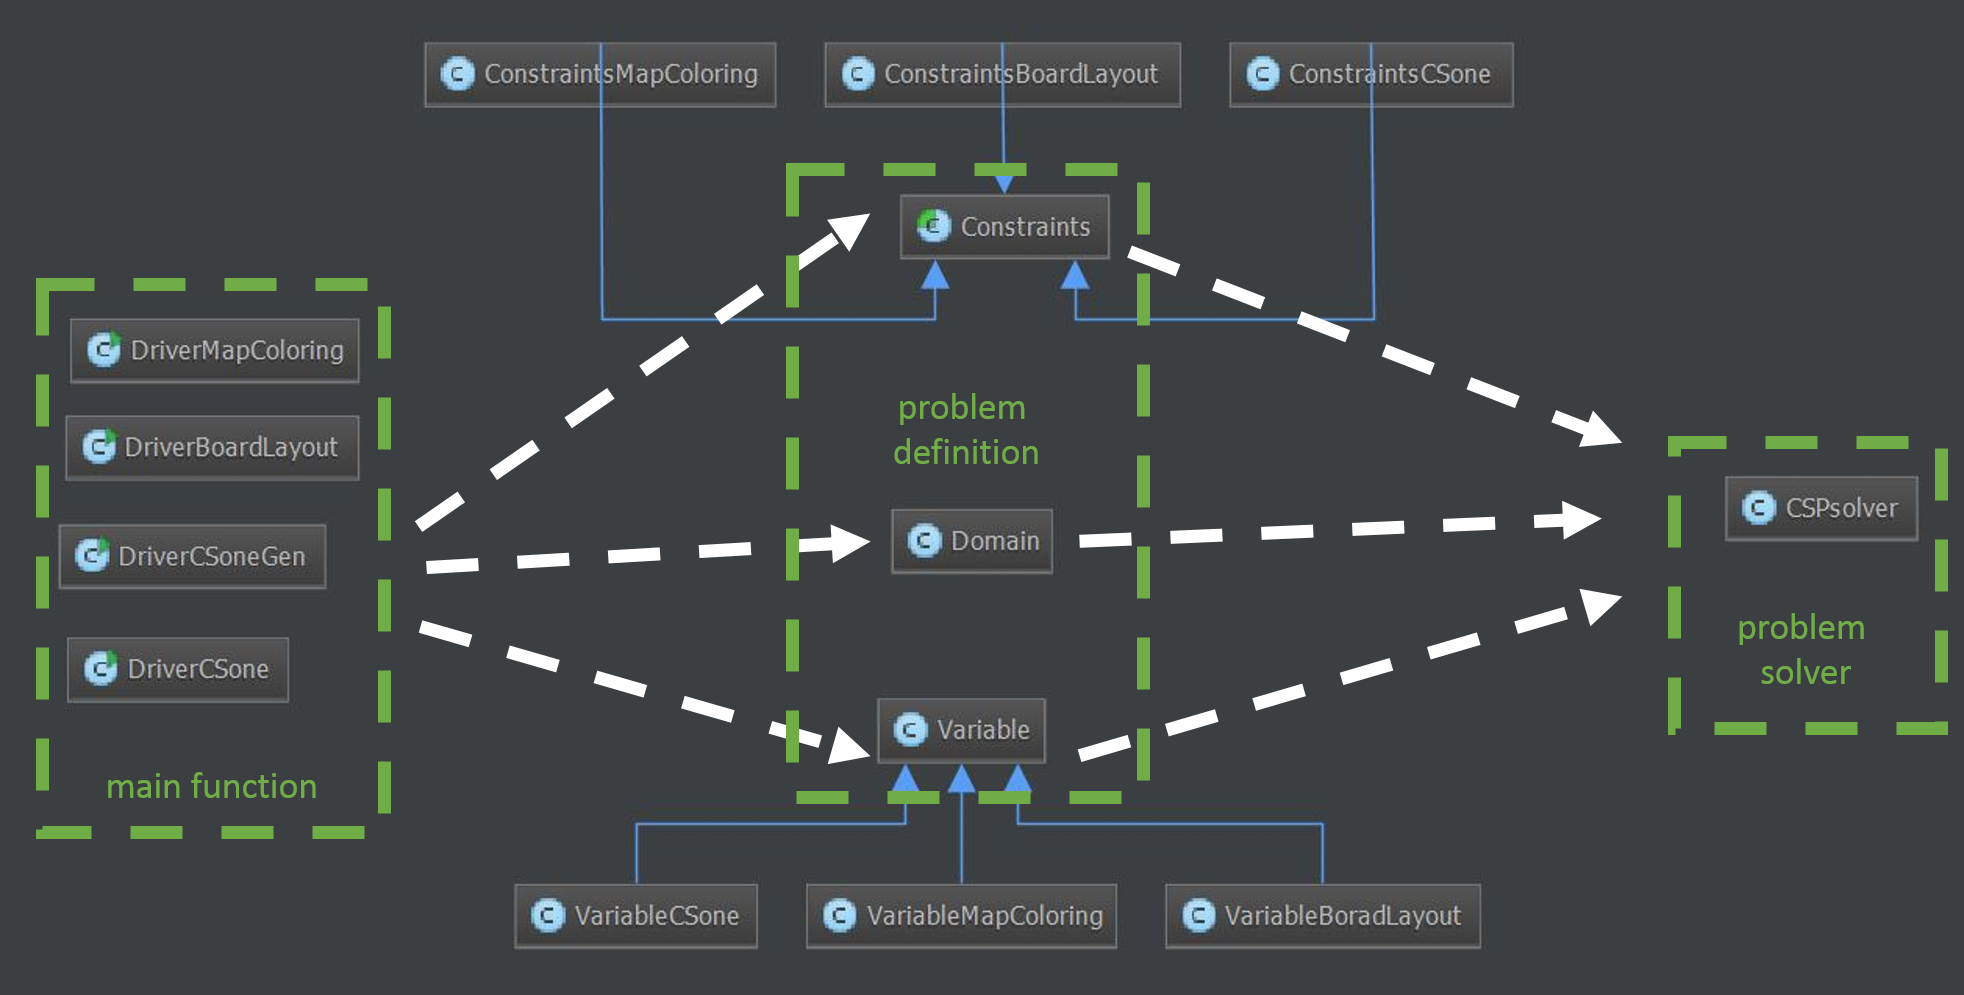
\includegraphics[width=0.99\textwidth]{class_layout.png}
\caption{Overview of the design}
\label{classlayout}
\end{figure*}




















\clearpage
\section{CSP solver}
\subsection{back-tracking}

\textbf{cspDFS} is a recursive style DFS method, which is the outline of the whole back-tracking. The basic procedure is,

\begin{enumerate}
  \item  Pick a \emph{variable} from the unassigned variable set;
  \item And then update all its valid \emph{domain} values;
  \item After preparation, it pick a \emph{domain} value, and keep recursion of the remaining \emph{variables}. Noted that if its successor report failure of DFS, it will iteratively choose the next \emph{domain} values;
\item   If it runs out of \emph{domain} values, it will undo the assignemnt and report fail of search to its parent.
\end{enumerate}

You may already notice some method names such as \textbf{pickMRV}, \textbf{sortLCV} and \textbf{MAC3Inference}. They are optimizations of the back-tracking algorithm, which will be explained in details later.

\begin{lstlisting}[numbers=left, caption=CSPsolver.class]
/**
 * @param remain: list of variables that is not assigned yet
 * @return: whether the search is successful or not
 */
protected boolean cspDFS(LinkedList<Variable> remain) {
  // base case of recursion
  if (remain.size() == 0) return true;
  // pick a Minimum Remaining Variable
  Variable var = pickMRV(remain);
  // update domain and sort the values based on Least Constraining
  sortLCV(var, remain);
  // iterate all the valid domain
  for (Domain domain : var.getDomains()) {
    var.assign(domain);
    // try to assign the next variable in the remain
    if (MAC3Inference(var, remain)) {
      if (cspDFS(remain)) {
        return true;  // solution found!
      }
    }
  }
  // not found, reset assignment and put variable back to remain
  undoAssignment(var, remain);
  return false;
}
\end{lstlisting}





\clearpage
\subsection{pickMRV}

The body of \textbf{pickMRV} is fairly simple: it returns the variable with min heuristic based on MRV heuristic.

\begin{lstlisting}[numbers=left, caption=CSPsolver.class]   
protected Variable pickMRV(LinkedList<Variable> remain) {
  Variable var = Collections.min(remain);
  remain.remove(var);
  return var;
}
\end{lstlisting}

The Main idea of MRV heuristic (minimum remaining values), is to find a variable with minimum remaining values, because these kind of value is most likely to cause a fail search. If two variable has the same amount of domain values, we pick the one with larger \emph{degree}, because potentially it also more easy to fail.

\begin{lstlisting}[numbers=left, caption=CSPsolver.class]    
@Override
public int compareTo(Variable o) {
  int compared = (int) Math.signum(domainSize() - o.domainSize());
  if(compared != 0)
    // return the one with minimum remaining values
    return compared;
  else
    // return the one with maximum degree
    return (int) Math.signum(o.getDegree() - getDegree());
}
\end{lstlisting}

\subsection{sortLCV}

\textbf{sortLCV} is bascially sort all the valid domain values based LCV heuristic(least constraint value). The key idea is to left domains for the remainning variables as much as possible, so that the search is more likely to succeed earlier.

\begin{lstlisting}[numbers=left, caption=CSPsolver.class]   
protected void sortLCV(Variable var, LinkedList<Variable> remain) {
  // update the remaining domains based on constraints
  updateDomains(var);
  // compute value heuristic by trying
  for (Domain domain : var.getDomains()) {
    var.assign(domain);
    // try to assign the next variable in the remain
    domain.h = 0.;
    // compute its effect on the remaining varaibles
    for (Variable v : remain)
      domain.h += remainingDomains(v);
  }
  var.undoAssign();
  Collections.sort(var.getDomains());
}
\end{lstlisting}









\clearpage
\subsection{MAC3Inference}

The body of \textbf{MAC3Inference} prunes the domains and forecast failure by checking arc consistency recursively. Supposed current variable is $X_i$. Line 5 means getting all the arcs $<X_i, X_j>$, where $\{X_j\}$ is the neighbors of $X_i$. Line 13 means getting all the $<X_k, X_i>$, where $\{X_k\}$ is the neighbors of $X_i$ except $X_j$.

This recursion of inference is meant to converge / terminate at some point.  Because it keeping pruning down the domains of the whole variables set, and stops recursion when no more domains can be pruned down. Since domain is a finite set, this inference is expected to termiante.

\begin{lstlisting}[numbers=left, caption=CSPsolver.class]  
protected boolean MAC3Inference(Variable thisVar,LinkedList<Variable> remain){
  // back up the properties of this variable
  Variable var = thisVar.snapshot();
  int backup = thisVar.getAssignment();
  LinkedList<Constraints.ArcPair> arcs = cons.getAdjArcs(var, remain);

  while (arcs != null && !arcs.isEmpty()) {
    Constraints.ArcPair arc = arcs.removeFirst();
    if (revise(arc.first, arc.second)) {
      if (var.getDomains().isEmpty())
        return false;
      arcs.addAll(cons.getAdjArcsInvert(arc.first, arc.second, remain));
    }
  }
  // recover properties of this variable
  thisVar.assign(new Domain(backup));
  return true;
}
\end{lstlisting}

The revise function prunes the domain when inconsistency occurs, and report the change of domains.

\begin{lstlisting}[numbers=left, caption=CSPsolver.class]   
protected boolean revise(Variable var, Variable adj) {
  for (Iterator<Domain> it = var.getDomains().iterator(); it.hasNext(); ) {
    // try to assign a domain and test if conflict exists
    var.assign(it.next());
    if (!cons.consistentTest(var, adj)) {
      it.remove();
      var.undoAssign();
      return true;
    }
  }
  var.undoAssign();
  return false;
}
\end{lstlisting}














\clearpage
\section{Problem definition}
Here I am presenting the outlines of two major classes that define the problem.

\subsection{Variable.class}

Here you can see the outline of \textbf{Variable}. Since most of the methods are very trivial, I am not presenting the details here.



\begin{table}[h]
\begin{center}
  \begin{tabular}{ |r | l | }
    \hline
    Modifier and Type & Field and Description \\ \hline
    protected int &	assignment                          \\ \hline
protected Constraints &	cons                            \\ \hline
protected int &	degree                                  \\ \hline
protected java.util.LinkedList$<$Domain$>$ &	domains       \\ \hline
protected java.util.LinkedList$<$Domain$>$ &	domainsBackup \\ \hline
protected int &	id \\ \hline

  \end{tabular}
\caption{Field Summary}
\end{center}
\end{table}


\begin{table}[h]
\begin{center}
  \begin{tabular}{| r | l|  }
    \hline
    Modifier and Type & Field and Description \\ \hline
    protected int &	assignment                          \\ \hline
  boolean	&assign(Domain domain)                     \\ \hline
int&	compareTo(Variable o)                          \\ \hline
int	&domainSize()                                    \\ \hline
void&	domainsRecover()                               \\ \hline
boolean&	equals(java.lang.Object other)             \\ \hline
int	&getAssignment()                                 \\ \hline
int	&getDegree()                                     \\ \hline
java.util.LinkedList$<$Domain$>$	&getDomains()          \\ \hline
int&	getId()                                        \\ \hline
java.util.ArrayList$<$java.lang.Integer$>$&	getStates()  \\ \hline
int&	hashCode()                                     \\ \hline
void	&setDegree(int d)                              \\ \hline
void	&setDomainsBackup()                            \\ \hline
Variable	&snapshot()                                \\ \hline
java.lang.String&	toString()                         \\ \hline
void	&undoAssign()                                  \\ \hline
    \hline
  \end{tabular}
\caption{Method Summary}
\end{center}
\end{table}


\subsection{Domain.class}
Domains is very simple, basically just domain value along with a heuristic value.


\clearpage
\subsection{Constraints.class}

Here you can see the outline of \textbf{Variable}. There are two basic members in this class. \textbf{binaryAdjs} is used to store all the binary relationship, whole \textbf{binaryAdjs} is for global relationships. I don't store the relationship such as equal, greater, etc. Assuming that all the arcs/sets have the same relationship. Of course you can extend members base on your need of problem. For example, if different binary constraints have different relationship, you should implement a hashmap from collection of variables to their relationship.



\begin{table}[h]
\begin{center}
  \begin{tabular}{ |r | l | }
    \hline
    Modifier and Type & Field and Description \\ \hline
static java.util.HashMap$<$Variable,java.util.LinkedList$<$Variable$>$$>$	&binaryAdjs  \\ \hline
static java.util.HashMap$<$java.lang.Integer,java.util.HashSet$<$Variable$>$$>$	&globalAdjs  \\ \hline

  \end{tabular}
\caption{Field Summary}
\end{center}
\end{table}




\begin{table}[h]
\begin{center}
  \begin{tabular}{ |r | l | }
    \hline
    Modifier and Type & Field and Description \\ \hline
void	&addConstraint(Variable var1, Variable var2)                                                                                   \\ \hline
void	&addGlobalVar(Variable var)                                                                                                    \\ \hline
boolean	&conflictTest(java.util.LinkedList$<$Variable$>$ vars)                                                                           \\ \hline
boolean	&conflictTest(Variable var)                                                                                                  \\ \hline
boolean	&consistentTest(Variable var, Variable adj)                                                                                  \\ \hline
LinkedList$<$Constraints.ArcPair$>$&	getAdjArcs(Variable var, LinkedList$<$Variable$>$ remain)                          \\ \hline
LinkedList$<$Constraints.ArcPair$>$	&getAdjArcsInvert(Variable var, Variable exclude, LinkedList$<$Variable$>$ remain)   \\ \hline
abstract boolean&	isSatisfied(Variable var1, Variable var2)                                                                          \\ \hline
void	&rmGlobalVar(Variable var)                                                                                                     \\ \hline

  \end{tabular}
\caption{Method Summary}
\end{center}
\end{table}

One major method is \textbf{conflictTest}. It is used to test conflict with the adjacent, after assigning values to a variable. The base method is written for binary constraint, because theoretically all problems can be represented by binary constraint problem. I will extend this for global constraints in some other problems, which makes the implementation and compuation more easy.

\begin{lstlisting}[numbers=left, caption=Constraints.class]   
/***
 * @param var: the variable to be tested
 * @return: whether the conflict exists
 */
public boolean conflictTest(Variable var) {
  LinkedList<Variable> adjs = binaryAdjs.get(var);
  if (adjs == null)
    return false; // no adjacent in constraint graph, no conflict
  for (Variable adj : adjs) {
    if (!isSatisfied(var, adj) ) 
      return true;
  }
  return false;
}
\end{lstlisting}



Since most of the methods are not very crucial, I am not presenting the details here. The most important one is the \textbf{isSatisfied} method. It related to specific problem, I will present those extended codes when discussing real problem application later.
















\clearpage
\section{Map coloring problem}
Map coloring is a very classic constraint satisfied problem. The basic idea is, any adjacent areas in the map should have different color, which forms a binary contraint.

\subsection{Important methods}
\textbf{isSatisfied} is method to determine whether two variables satisfied the bianry constraint. For each assigment, there can be a list of states corresponding to this vairble. The \textbf{getStates} is such a genric method in the base class. As you can see for map coloring problem, there is only one states, which is the assigned color.

Depending on the needs of the problem, I will override the \textbf{getStates} in \textbf{VariableExtendClass}, and wrote corresponding \textbf{isSatisfied} in the \textbf{ConstraintsExtendClass}

\begin{lstlisting}[numbers=left, caption=ConstraintsMapColoring.class]   
@Override
public boolean isSatisfied(Variable var1, Variable var2){
    return var1.getStates().get(0) != var2.getStates().get(0);
}
\end{lstlisting}

\begin{lstlisting}[numbers=left, caption=VariableMapColoring.class]   
public ArrayList<Integer> getStates() {
    return new ArrayList<>(Arrays.asList(getAssignment()));
}
\end{lstlisting}


\subsection{Testing}
The following list the the results of Austrilia coloring, with constriants described by figure \ref{aus}\footnote{from Artificial Intelligence A Modern Approach 3rd Edition}

\begin{lstlisting}[numbers=left]   
[WA->Yellow]
[NT->Red]
[SA->Green]
[Q->Yellow]
[NSW->Red]
[V->Yellow]
[T->Red]
\end{lstlisting}

\begin{figure*}[!h]
\centering
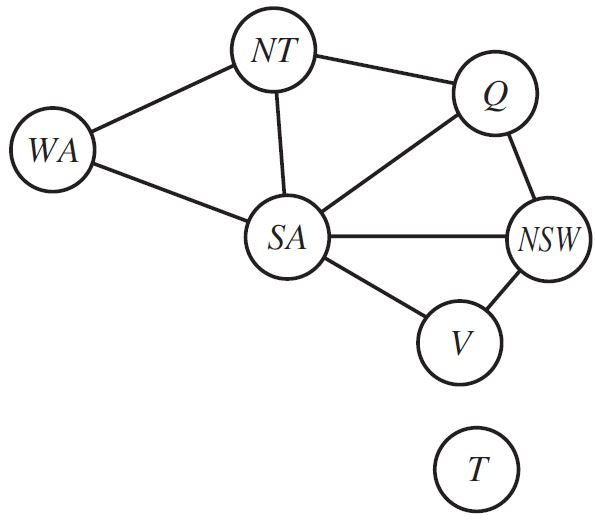
\includegraphics[width=0.25\textwidth]{austrilia.jpg}
\caption{Constraint graph of Austrilia map coloring problem. }
\label{aus}
\end{figure*}

I also test the solver on US States coloring. \footnote{thanks to data this website help me to build the constraint graph.  \url{http://writeonly.wordpress.com/2009/03/20/adjacency-list-of-states-of-the-united-states-us/}} Here comes the results.

\begin{lstlisting}[numbers=left]   
[AK->Red]
[AL->Yellow]
[AR->Yellow]
[AZ->Yellow]
[CA->Red]
[CO->Green]
[CT->Green]
[DC->Yellow]
[DE->Green]
[FL->Red]
[GA->Green]
[HI->Red]
[IA->Yellow]
[ID->Green]
[IL->Red]
[IN->Green]
[KS->Yellow]
[KY->Yellow]
[LA->Red]
[MA->Yellow]
[MD->Red]
[ME->Yellow]
[MI->Yellow]
[MN->Red]
[MO->Green]
[MS->Green]
[MT->Red]
[NC->Yellow]
[ND->Yellow]
[NE->Red]
[NH->Red]
[NJ->blue]
[NM->blue]
[NV->blue]
[NY->Red]
[OH->Red]
[OK->Red]
[OR->Yellow]
[PA->Yellow]
[RI->Red]
[SC->Red]
[SD->Green]
[TN->Red]
[TX->Green]
[UT->Red]
[VA->Green]
[VT->Green]
[WA->Red]
[WI->Green]
[WV->blue]
[WY->Yellow]
\end{lstlisting}

This is a much more complex coloring problem, where I can give more analysis on the performance of my CSP solver, as figure \ref{mapcoloring} shows. 

To my surprise, using LCV alone makes the search twice as worse as back tracking. But combining MRV and LCV heuristic together does get the best performance, indicating that LCV can have positive influence. I guess the reason why LCV alone performance worst, is because it keep using the values that is least likely to cause failure. Turn out that it waste too much time on those variables that needs massive search while being exploered too early. (Because I am not using MRV here).

As you can see, MAC3 explore the same amount of nodes as back tracking does. However it cause slightly more time because it needs to compute the inference. The reason that MAC3 has no effect is because arc consistency is not effective on map coloring problem. In this case we should use other method such as path consistency. I will leave to future work.

\begin{figure*}[!h]
\normalsize
\centering
\subfigure[time]{
\label{m-1-3} %% label for first subfigure
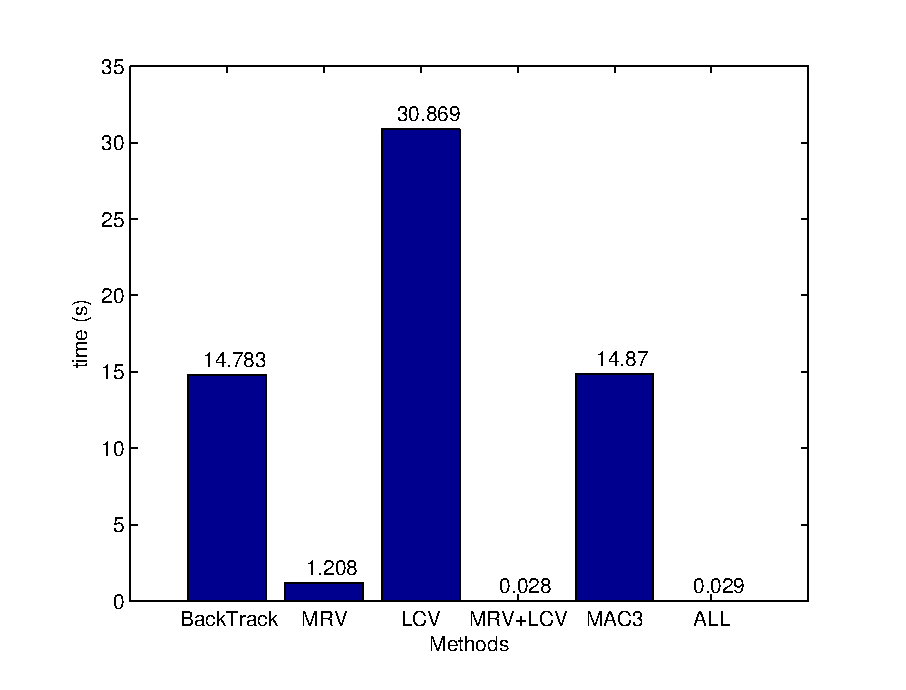
\includegraphics[width=0.48\textwidth]{mapcoloring.eps}}
\subfigure[nodes]{
\label{m-1-0} %% label for second subfigure
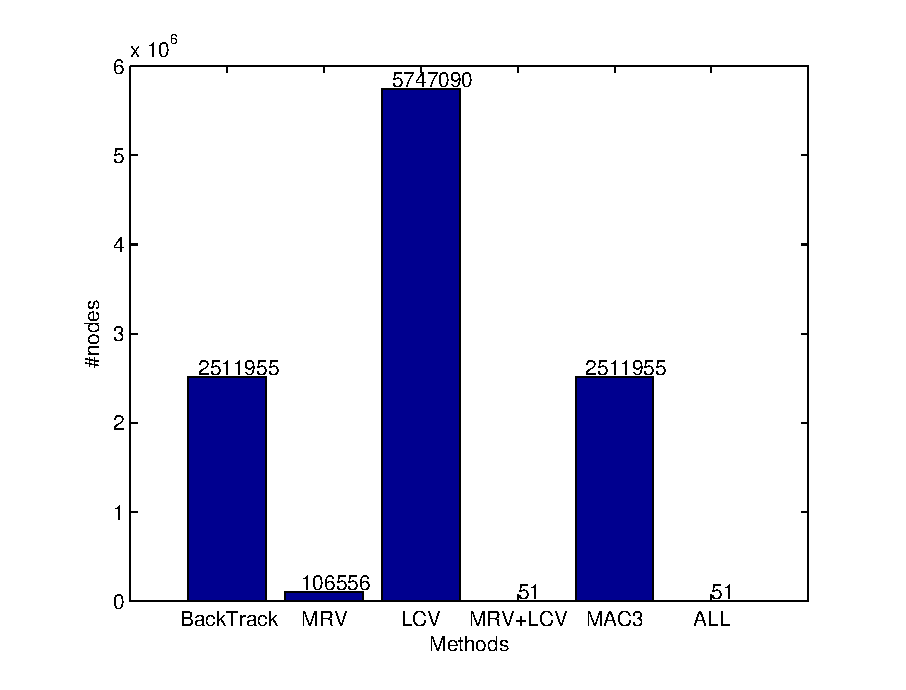
\includegraphics[width=0.48\textwidth]{mapcoloringnodes.eps}}
\caption{Performance comparison between different methods.}
\label{mapcoloring} %% label for entire figure
\end{figure*}











\clearpage
\section{Circuit board layout problem}
Circuit board is another classic problem that can be described bt binary constraints. The basic idea is that two layouts should not \emph{overlap } with each other. So, based on my previous work on map coloring, the only thing I need to do is to add a few members and methods to \emph{VariableBoardLayout}, as well as implement the \textbf{isSatisfied} abstract method.

The domains of this problem is the locations of the components. Basically I use the following formula to convert the location into the integer that can be used by my CSP solver. The $OFFSET$ is defined inside VariableBoradLayout.class. I set it to 1000 when I test the code.

$$x * VariableBoradLayout.OFFSET + y$$

\subsection{Important methods}


Let's say I have a component that is $w\times h$, with a $m\times n$ board , and the bottom-left point represent the position of the component. Initially, the domains (position) of this component should be $\{(x, y)\}, $ where $ x\in [0, n - w] $ and $ y\in [0, m - h].$


\begin{lstlisting}[numbers=left, caption=DriverBoardLayout.class] 
...
// initiate domain
domains = new LinkedList<>();
for (int x = 0; x <= domainRange.w - rects.get(i).w; x++) {
  for (int y = 0; y <= domainRange.h - rects.get(i).h; y++) {
    domains.add(new Domain(x * VariableBoradLayout.OFFSET + y));
  }
}
...
\end{lstlisting}



As you can see, \textbf{isSatisfied} and \textbf{getStates} are more complex than the previous one. The basic idea is to get the pixels location of the one rectanle, and store each pixel into a hashset. And then I traverse through the other rectangle and see if any one already exists in the hash set. The time complexity is $O(m + n)$, where $m$ and $n$ is the size of these two shape.

Currently the getState imply that the shape is a rectangle, by doing I can save some memory. I can implemente VariableBoradLayout.class instead of using mathematical calculation in order to makes it scalable to any kind of shapes.

 

\begin{lstlisting}[numbers=left, caption=ConstraintsBoardLayout.class] 
@Override
public boolean isSatisfied(Variable var1, Variable var2){
  HashSet<Integer> overlap = new HashSet<>();
  ArrayList<Integer> states1 = var1.getStates();
  ArrayList<Integer> states2 = var2.getStates();
  for(Iterator<Integer> it = states1.iterator(); it.hasNext();){
    overlap.add(it.next());
  }
  for(Iterator<Integer> it = states2.iterator(); it.hasNext();){
    if(overlap.contains(it.next()))
      return false;
  }
  return true;
}
\end{lstlisting}

\begin{lstlisting}[numbers=left , caption=VariableBoradLayout.class]   
@Override
public ArrayList<Integer> getStates() {
  ArrayList<Integer> states = new ArrayList<>();
  for(int i = 0; i < width; i++){
    for(int j = 0; j < height; j++){
      states.add(getPixel(i, j));
    }
  }
  return states;
}
\end{lstlisting}


\subsection{Testing}
First I test the following example in a $10\times3$ board. The result is shown as figure \ref{boardlayout}, where the white area represent the board. 
\begin{lstlisting}[numbers=left]   
      bbbbb   cc
aaa   bbbbb   cc  eeeeeee
aaa           cc 

..........
..........
..........
\end{lstlisting}

\begin{figure*}[!h]
\centering
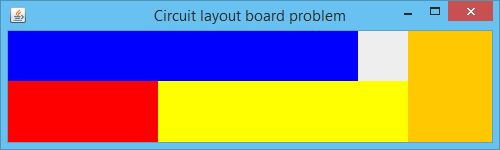
\includegraphics[width=0.49\textwidth]{boardlayout.JPG}
\caption{Overview of the design}
\label{boardlayout}
\end{figure*}









\section{CS 1 section assignment problem}















\section{Map coloring problem}
Map coloring is a very classic constraint satisfied problem. The basic idea is, any adjacent areas in the map should have different color, which forms a binary contraint.

\subsection{Important methods}
\textbf{isSatisfied} is method to determine whether two variables satisfied the bianry constraint. For each assigment, there can be a list of states corresponding to this vairble. The \textbf{getStates} is such a genric method in the base class. As you can see for map coloring problem, there is only one states, which is the assigned color.

Depending on the needs of the problem, I will override the \textbf{getStates} in \textbf{VariableExtendClass}, and wrote corresponding \textbf{isSatisfied} in the \textbf{ConstraintsExtendClass}
\begin{lstlisting}[numbers=left]   
@Override
public boolean isSatisfied(Variable var1, Variable var2){
    return var1.getStates().get(0) != var2.getStates().get(0);
}
\end{lstlisting}


















\subsubsection{minimaxIDS}

\textbf{minimaxIDS} initializes the search using iterative-depending strategy.


\begin{lstlisting}[numbers=left]
private short minimaxIDS(Position position, int maxDepth) 
    throws IllegalMoveException{
  this.terminalFound = false;
  MoveValuePair bestMove = new MoveValuePair();
  for (int d = 1; d <= maxDepth && !this.terminalFound; d++) {
    bestMove = maxMinValue(position, maxDepth - 1, MAX_TURN);
  }
  return bestMove.move;
}
\end{lstlisting}


\subsubsection{maxMinValue}

\textbf{maxMinValue} is an recursive funciton that keep searching in the tree. I write it in a compact way by mering min and max procedure in this one method, which turns out to be a big mistake for future when I try to implement more fancy mechansim for the searching. This design makes the codes a little messy.

There is also another better way to implement the search in a compact way, which is called \emph{Nagamax}. However it was too late for me to discover it so I leave it to my future work.

\begin{lstlisting}[numbers=left]
private MoveValuePair maxMinValue(Position position, int depth, 
    boolean maxTurn) throws IllegalMoveException{
  if (depth <= 0 || position.isTerminal()) {
    // the base case of recursion
    return handleTerminal(position, maxTurn);
  } else {
    // get all the legal moves
    MoveValuePair bestMove = new MoveValuePair();
    for (short move : position.getAllMoves()) {
      // collect values from further moves by recursion
      position.doMove(move);
      MoveValuePair childMove = maxMinValue(position, depth - 1, !maxTurn);
      bestMove.updateMinMax(move, childMove.eval, maxTurn);
      position.undoMove();
    }
    return bestMove;
  }
}
\end{lstlisting}

\subsubsection{handleTerminal}

\textbf{handleTerminal} is used to terminate the searching by returning an evalution value, when either reaching the maximun depth or check mate or draw. Noted that getMaterial evalutes the weighted sum of the stones, while getDominant evaluates the distribution of the stones.

\begin{lstlisting}[numbers=left]
private MoveValuePair handleTerminal(Position position, boolean maxTurn) {
  MoveValuePair finalMove = new MoveValuePair();
  if (position.isTerminal() && position.isMate()) {
    this.terminalFound = position.isTerminal();
    finalMove.eval = (maxTurn ? BE_MATED : MATE);
  } else if (position.isTerminal() && position.isStaleMate())
     finalMove.eval = 0;
  else {
    finalMove.eval = (int) ( (maxTurn ? 1 : -1) * (position.getMaterial() 
       + position.getDomination()));
  }
  return finalMove;
}
\end{lstlisting}

\subsubsection{helper class}

\textbf{MoveValuePair} help me to store the move and corresponding evaluation value. Also it has a generalized method that help me to find the max value for maximum search, or vise versa.

\begin{lstlisting}[numbers=left]
private MoveValuePair handleTerminal(Position position, boolean maxTurn) {
  MoveValuePair finalMove = new MoveValuePair();
  if (position.isTerminal() && position.isMate()) {
    this.terminalFound = position.isTerminal();
    finalMove.eval = (maxTurn ? BE_MATED : MATE);
  } else if (position.isTerminal() && position.isStaleMate())
     finalMove.eval = 0;
  else {
    finalMove.eval = (maxTurn ? 1 : -1) * position.getMaterial();
  }
  return finalMove;
}
\end{lstlisting}





























\clearpage
\section{Results demonstration}


I did a lot of testing, turn out that I don't leave myself much time to organize how to present them. Here I am going to focus on computation time of each step. I create a fix random seed for the random AI, and let my AI play with it. 

Figure \ref{miniab} demonstrate the step and time curve, with my Minimax against Random AI (blue curve),  $\alpha\beta$ pruning against Random AI respectively (green curve). The left figure is a normal plot, while y axis of the right one is set to log scale (Noted that logy scale will shrink the difference on $y$ direction!). Considering sometimes the computation time grows exponentially with depth, this can provide a better observation. As you can see, the $\alpha\beta$ pruning finish the game using exact same amount of steps, while taking much less computation time.

\begin{figure*}[!h]
% ensure that we have normalsize text
\normalsize
% Store the current equation number.
% Set the equation number to one less than the one
% desired for the first equation here.
% The value here will have to changed if equations
% are added or removed prior to the place these
% equations are referenced in the main text.
\centering
\subfigure[normal]{
\label{m-1-3} %% label for first subfigure
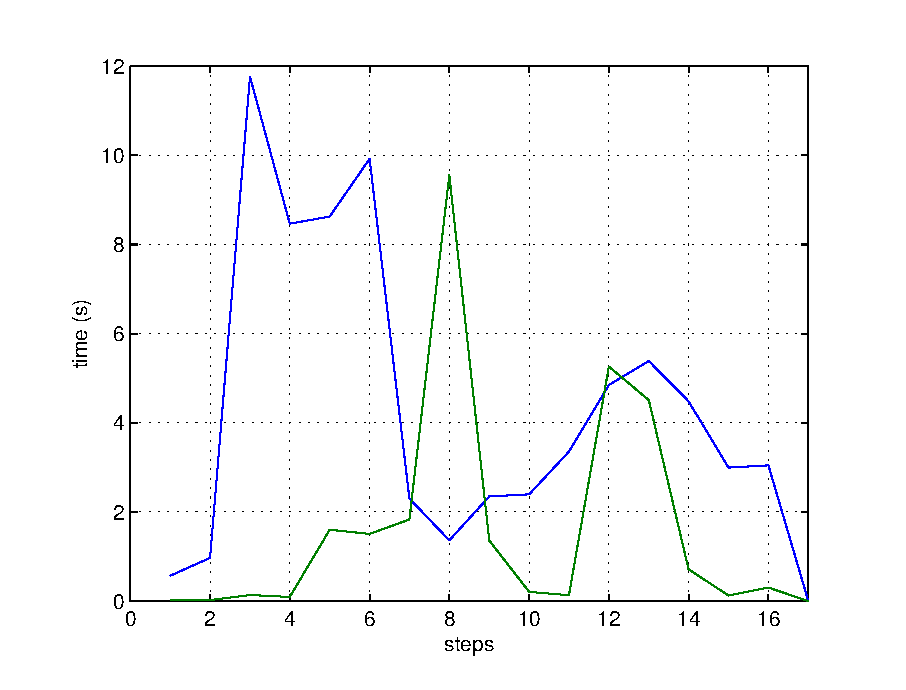
\includegraphics[width=0.48\textwidth]{mini_ab.eps}}
\subfigure[log scale]{
\label{m-1-0} %% label for second subfigure
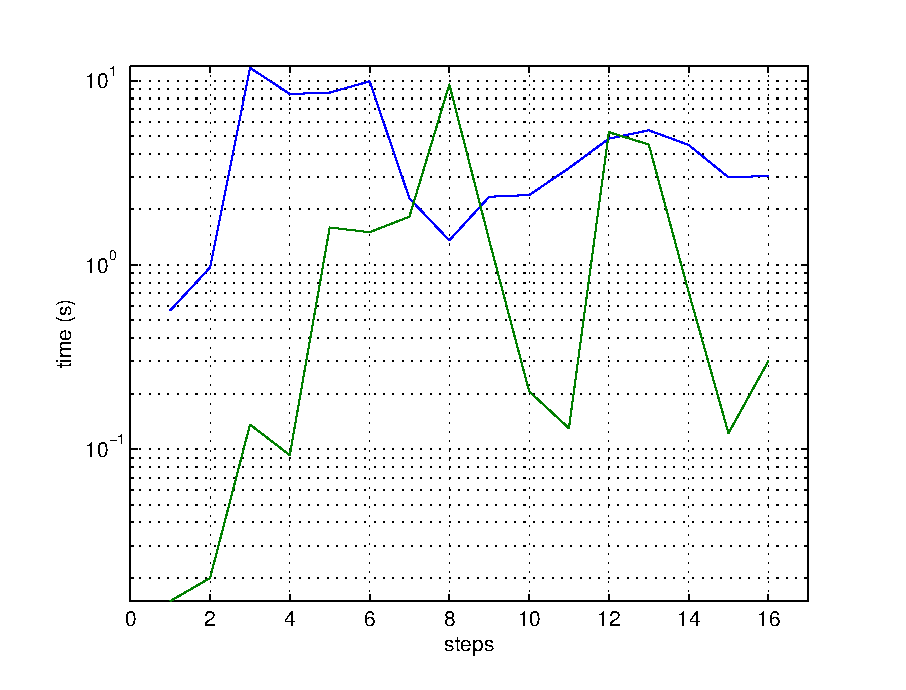
\includegraphics[width=0.48\textwidth]{mini_ab2.eps}}
\caption{step and time curve of Random MinimaxAI and $\alpha\beta$ pruning.}
\label{miniab} %% label for entire figure
\end{figure*}

Figure \ref{abtrans} demonstrate the step and time curve difference when there exists a tranposition table. As expected, the time conusmption is lower when implemented with transposition table. What's more, with transposition table it actually finish the game even fater! Because sometimes the table provider more depth of information than current node, which might lead to a bette decision.

Figure \ref{transorder} demonstrate the step and time curve difference when there exists a tranposition table. Though the time decrease even more significantly, the takes more steps for some unknown reason. I also test ordering enhancement against pure transposition table, it shows that after reodering it becomes a little more stupid. This leave as my future work.

Figure \ref{meantime} demonstrate mean time of different methods. It seems that null-move actually takes more time. I think it becuase although it reduce depth of search occassionally, it actually increase searching times on the same depth. May be I haven't tuned it properly. 

\begin{figure*}[!h]
\centering
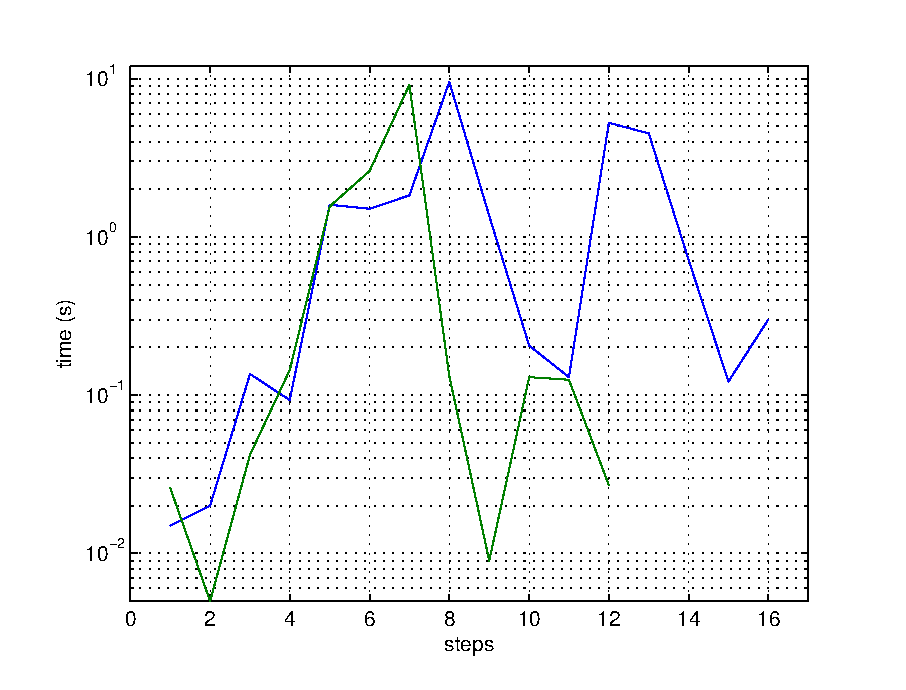
\includegraphics[width=0.48\textwidth]{mini_trans.eps}
\caption{step and time curve of $\alpha\beta$ pruning and$\alpha\beta$ enhanced with transposition table }
\label{abtrans}
\end{figure*}

\begin{figure*}[!h]
\centering
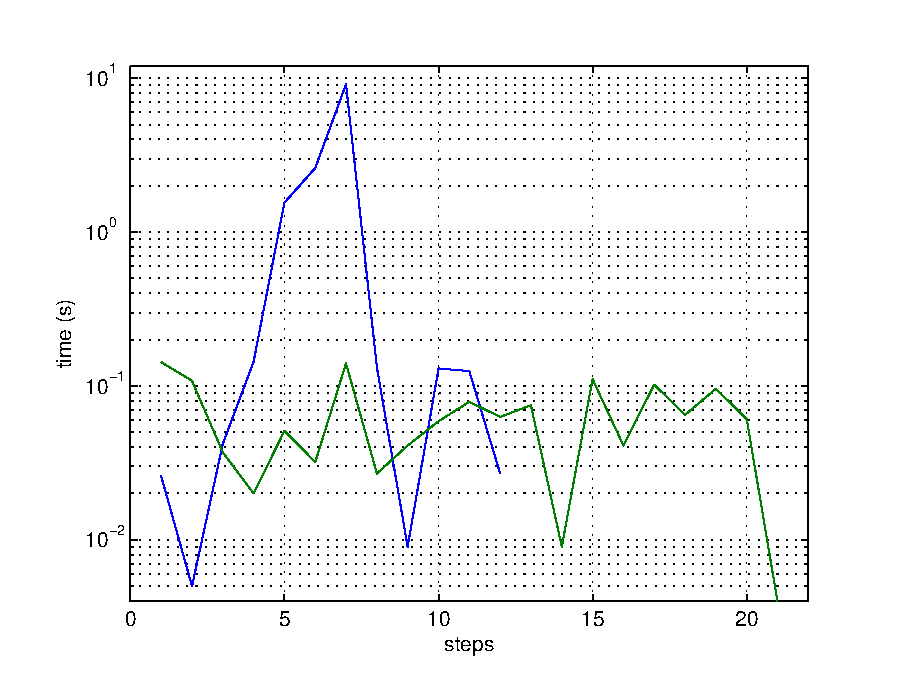
\includegraphics[width=0.48\textwidth]{trans_order.eps}
\caption{step and time curve of transposition table and$\alpha\beta$ enhanced with re-ordering}
\label{transorder}
\end{figure*}

\begin{figure*}[!h]
\centering
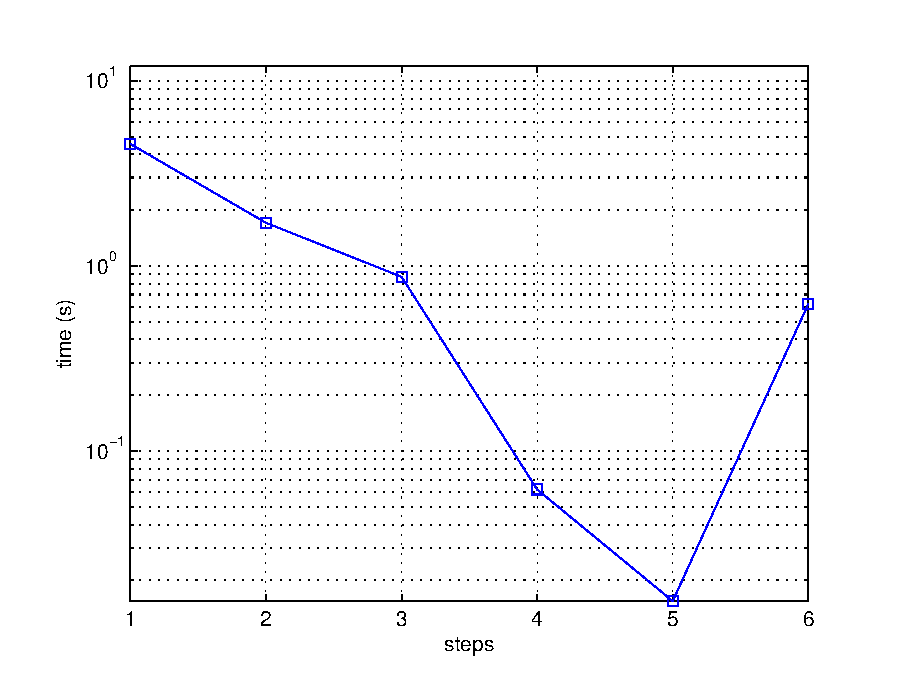
\includegraphics[width=0.48\textwidth]{meantime.eps}
\caption{mean time regards to Minimax, Alpha-beta pruning, transposition table, moves reodering, quiescence search and null move heuristic  repectively}
\label{meantime}
\end{figure*}


\clearpage
\section{Some related work}

Null move strategy can be very tricky. Adaptive Null-Move Pruning \footnote{Heinz, Ernst A. "Adaptive null-move pruning." Scalable Search in Computer Chess. Vieweg+ Teubner Verlag, 2000. 29-40.} prose some good suggestions. 1) when depth is less or equal to 6, use $R=2$. When Depth is larger than 8, use $R=3$. When depth is 6 or 7, and both sides has more than 3 stones, then $R = 3$. Otherwise, R = 2.




\end{document}